\chapter{Usage}
\section{User Interface}
I developed two user interfaces to interact with the tool, for now they are complementary and have not the same purpose but they interact in the same way with the core of the tool so making an other interfaces that does all the job can be easily done.
\subsection{CLI}
The \acrlong{cli} developed allows the user to help the algorithm to learn. It will be needed almost exclusively for learning and monitoring of the variables if needed. It prints everything that is happening in the execution of the tool, with a certain level of detail set by the user. You can see the CLI at start time on \autoref{fig:cli-start}. There are also example of the output produced by the \acrshort{cli} in Appendix \ref{section:cli-dumps}.
\begin{figure}
    \centering
    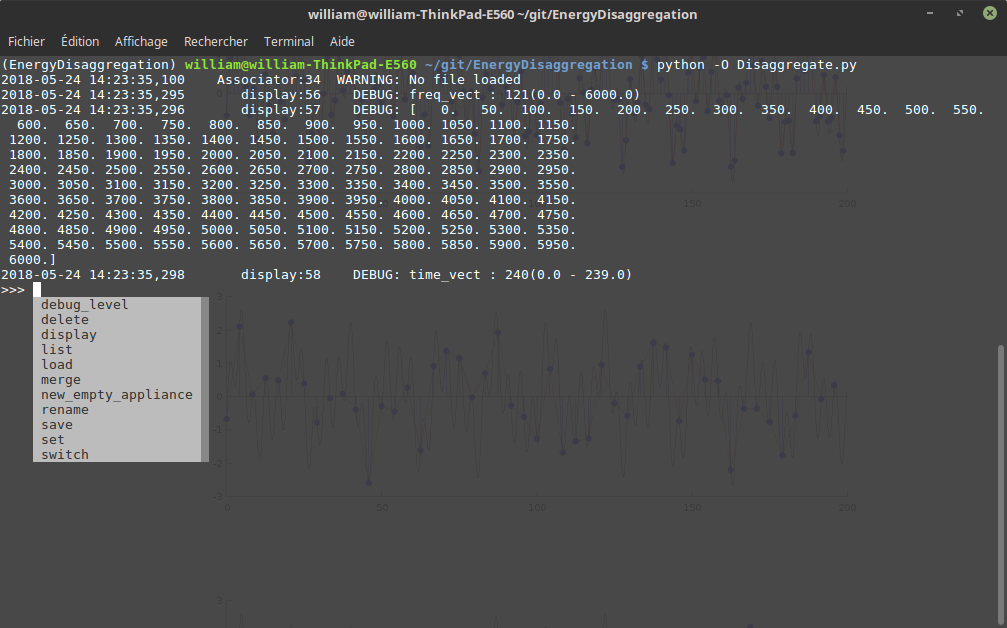
\includegraphics[width=\textwidth]{img/cli-start.png}
    \caption{The CLI at the start of the soft}
    \label{fig:cli-start}
\end{figure}

There are many things you can do to interract with the software. Here are the current commands :
\begin{description}
\item[\texttt{debug\_level}]This command allows to select the granularity level of text displayed by the tool. You can choose between \texttt{DEBUG}, \texttt{INFO}, \texttt{WARNING} and \texttt{ERROR}, where \texttt{DEBUG} displays everything that is happening, \texttt{INFO} shows only the useful info needed when the algorithm is already trained, and \texttt{WARNING} and \texttt{ERROR} only show minor and critical error, respectively.
\item[\texttt{delete}] When the algorithm doesn't recognise an appliance, it will not discard the data but create a new appliance with the data associated. This command allows to delete that appliance if it was indeed noise or something unwanted.
\item[\texttt{display}] This is used to launch the GUI if it wasn't started yet or if it was closed.
\item[\texttt{list}] This command list all the appliances known and their current state.
\item[\texttt{load}] You can use \texttt{load} to retrieve the information of an appliance you saved on a previous instance of the program.
\item[\texttt{merge}] You can group two appliances if you think they are similar and that the detection should not make a difference between those appliances.
\item[\texttt{new\_empty\_appliance}] When you try to add a new appliance on a system that already knows some appliances but the new appliance doesn't have a signal that is far enough from a known appliance, chances are that the algorithm will not create a new appliance but associate the new data to the existing appliance. To correct this, you can create a new appliance manually with this command.
\item[\texttt{rename}] Use this to rename an appliance if you don't want generic names like \texttt{item\_0}, \texttt{item\_1},...
\item[\texttt{save}] Once you have trained the algorithm to recognise an appliance, save it with this command in order to be able to recognise it too on other runs of the algorithm.
\item[\texttt{set}] If the algorithm didn't correctly recognise the change of state of an appliance, you may need to set it to its correct state manually with this command.
\item[\texttt{switch}] If the algorithm didn't classify correctly new data, it will assign it to a wrong appliance. You will need to switch it from the wrong appliance to the correct one with this command.
\end{description}

\subsection{GUI}
The \acrlong{gui} doesn't provide any functionality for now, but can be very useful to understand what is going on on the algorithm's mind.
\begin{figure}[t]
    \centering
    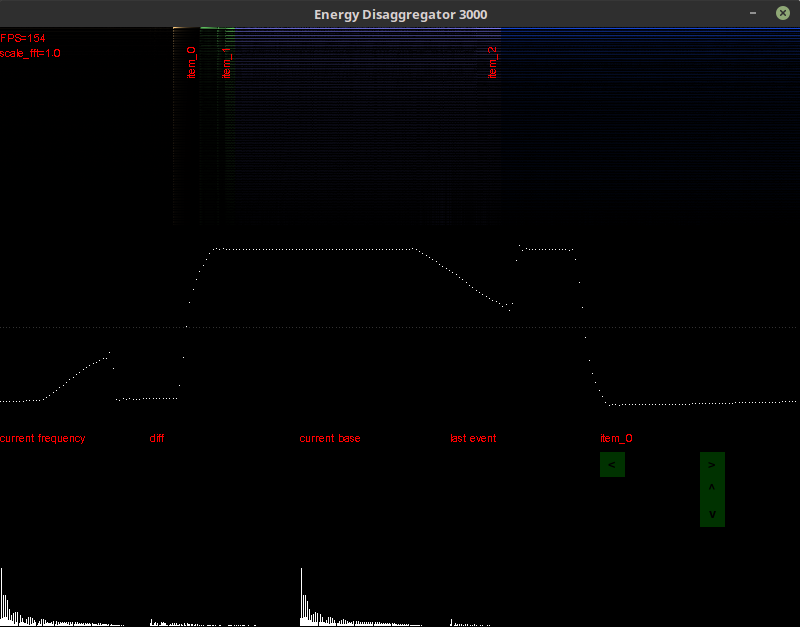
\includegraphics[width=\textwidth]{img/gui-start.png}
    \caption{The GUI at the start of the soft}
    \label{fig:gui-start}
\end{figure}
An screenshot is shown on \autoref{fig:gui-start}. It was taken a few seconds after the start of the algorithm, so nothing is really learned yet.

The screen is divided in multiple parts :
\begin{itemize}
    \item At the top there is a representation of the spectrogram of the electrical network. The top of the spectrogram represents the lower frequencies, and the top the upper frequencies. With the parameters used, the highest frequency we can see is 6kHz. The spectrogram slides with time to the left so that the right of the spectrogram always shows the most recent data. You can see that there are 3 tags on it, labelled \texttt{item\_0} through \texttt{item\_2}. These are the events detected by the algorithm, when it detected them. When an event is detected, the color of the spectrogram changes to give a better visualization.
    \item At the middle of the screen, a representation of the current wave going through the electrical network is represented. There is no interpolation made on the graph so that we see what the algorithm sees.
    \item On the bottom of the screen, there are multiple spectrum represented, from left to right :
    \begin{itemize}
        \item The first is the spectrum of the wave currently displayed at the middle of the screen.
        \item The third is the spectrum of the current base. As you will see if you run the program, this will converge to a stable point that is the mean of the few first readings after the base changes.
        \item The second is the absolute value of the difference between the base and the spectrum of last wave read.
        \item The fourth shows the last spectrum that was classified as being an appliance, i.e. the difference between the mean of signal read a few times and the base right before changing the base.
        \item The fifth displays the data recorded for the different appliances. There are buttons allowing you to choose which appliance it needs to display.
    \end{itemize}
    All these spectrum are made with a real Fourier transform, and only the absolute value of the real part is displayed.
\end{itemize}



\section{Communication with other software}
Because ultimately the main use of the algorithm is not just being able to disaggregate, there is an option allowing to output the states of the appliances on a listening port. We can for instance listen on a port with \texttt{netcat} and send the information with \texttt{python -O Disaggregate.py -p \$PORT -i \$IP}. Every time an event is detected, the appliance and its new state will be outputted on the port.

\section{Training}
In order to have the most accurate data possible, we should train the algorithm one appliance at the time, without anything else making noise. In order to do that, I altered an electrical power strip in order to be able to plug the sensor on it. There should be very few interference coming from the outside world and indeed, the GUI shows a flat line when nothing is plugged into the power strip.

The training doesn't take a lot of time per appliance, but it needs to be made manually for now. An idea of the general process is the following :
\begin{enumerate}
    \item Plug the new appliance into the power strip.
    \item Change the state of the appliance, lets call it state 1. An event should be detected and the algorithm will create a new appliance and put the data in it.
    \item Change the state of the appliance, lets call it state 2. Again, an event should be detected and an new appliance created.
    \item Switch the data from the last event into a new state of the first appliance.
    \item Set manually the state of the appliance to it's real state. Because you manually switched the data, the algorithm doesn't know that the appliance is in state 2 and it wont be able to detect state 1 at the next step. It is indeed not allowed to detect a state it is already in.
    \item Change the state to state 1. Now the algorithm should correctly assign the new data to the correct state of the appliance. If not, switch the data to its correct place and set the state manually.
    \item Change the state to state 2 and do the same as previously if the data is missclassified.
    \item Repeat the last two steps until there a no more errors and the k nearest neighbours are all from the correct state.
\end{enumerate}

However, in some cases we might need to adapt the manual corrections for some appliances because sometimes an appliance goes through multiple states when you make it go to another state.

\subsection{Different types of appliances}\label{section:appliances}
\subsubsection{Halogen lamp}
\begin{figure}
    \centering
    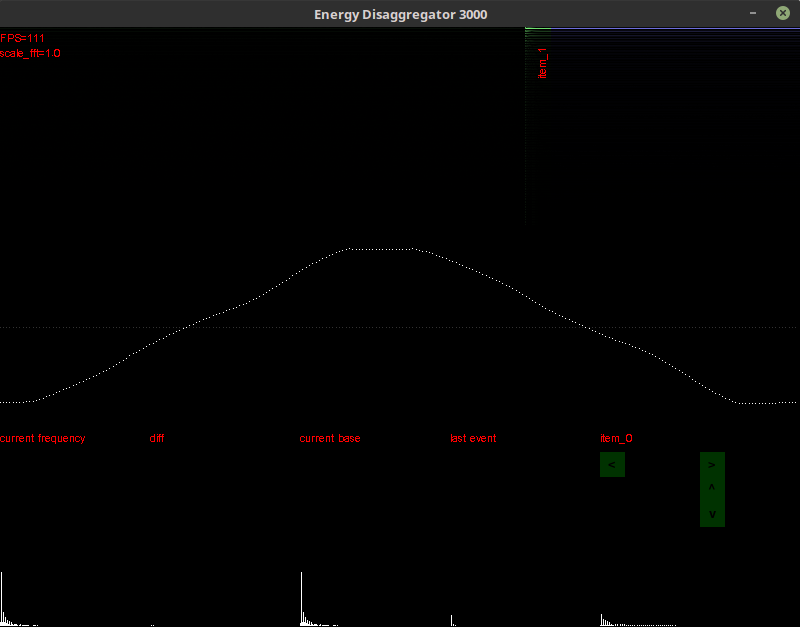
\includegraphics[trim={0 7cm 0 7cm},clip,width=\textwidth,decodearray={1 0 1 0 1 0}]{img/gui-halogen.png}
    \caption{Representation of the wave of an halogen lamp}
    \label{fig:gui-halogen}
\end{figure}
On \autoref{fig:gui-halogen} you can see the GUI displaying the wave and spectrum emitted by an halogen lamp. Without much surprise, this is very close to a sine wave because an halogen lamp is almost only resistive. However, we can see that the amplitude of the harmonics of 60Hz is not null.

The training of such a device is very easy as there are only two states : on and off.

\subsubsection{Compact Fluorescent Lamp (CFL)}
Now lets take a slightly more complex case : a \acrshort{cfl} lamp. Most of the appliances designed to save energy go through some kind of heating when we start them in order to load the capacitors and the inductor at the desired level.

You can see the wave when we just turned the light on on \autoref{fig:gui-cfl-start}, and when the heating is finished on \autoref{fig:gui-cfl-eco}.
\begin{figure}
\begin{subfigure}{\textwidth}
    \centering
    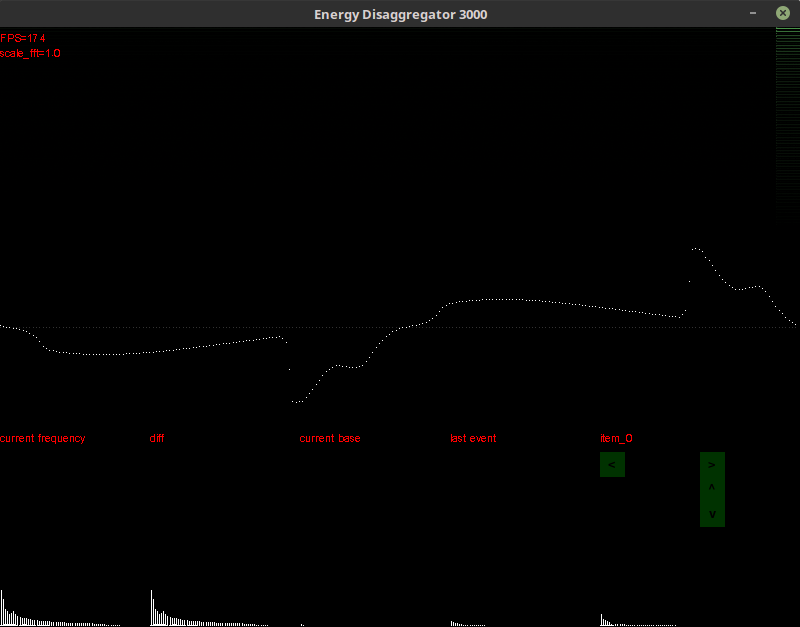
\includegraphics[trim={0 7cm 0 7cm},clip,width=\textwidth,decodearray={1 0 1 0 1 0}]{img/gui-cfl-start.png}
    \caption{Representation of the wave of a CFL at start}
    \label{fig:gui-cfl-start}
\end{subfigure}
\begin{subfigure}{\textwidth}
    \centering
    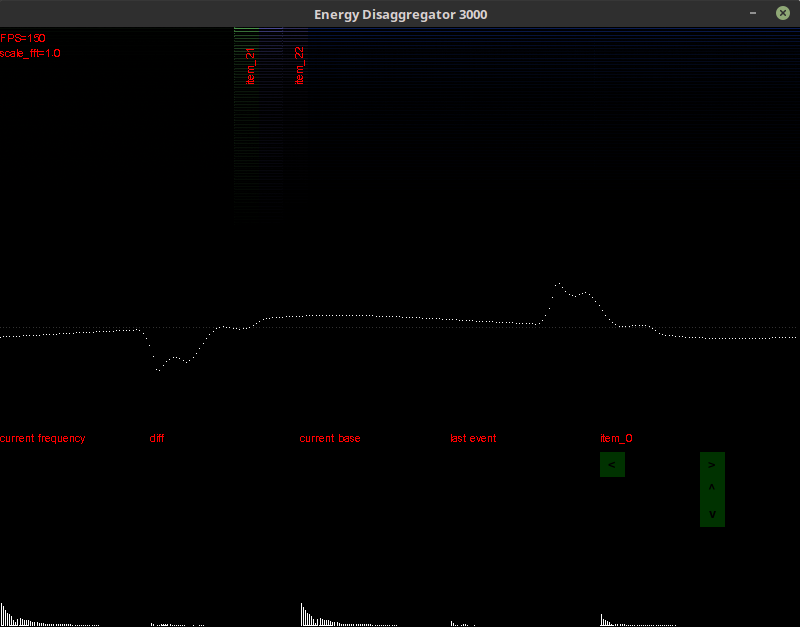
\includegraphics[trim={0 7cm 0 7cm},clip,width=\textwidth,decodearray={1 0 1 0 1 0}]{img/gui-cfl-eco.png}
    \caption{Representation of the wave of a CFL after warm up}
    \label{fig:gui-cfl-eco}
\end{subfigure}
\caption{Representation of the waves of the differetn states of a CFL}
\label{fig:gui-cfl}
\end{figure}
They are very similar, the main difference is the phase of the signal captured and the amplitude of the signal. The amplitude of all the frequencies seems to be halved with this particular lamp.

The interesting part in this is that when we turn on the lamp, the algorithm detects the two states above. This lamp will then have 3 states : on, eco, and off.

\subsubsection{Laptop charger}
Now lets take an even more complicated appliance : the laptop charger. The one I tested takes an input AC of 220V and 1.8A, and gives an output DC of 20V and 3.25A.
At first thought it might seem similar to a CFL, but actually there is a difference : we can plug it from both ends : one in the laptop and one in the electrical socket. This means there are at least 4 actions for this appliance, with one state per action. Actually there is a fifth state for the warm-up when we plug it into the laptop.

The different states can be seen on \autoref{fig:gui-laptop-start}, \autoref{fig:gui-laptop-eco} and \autoref{fig:gui-laptop-unplugged}. The states registered for this appliance are : when we plug the charger in the electrical socket without plugging it into the laptop, when we unplug the electrical socket, when we plug it in the laptop when it was already plugged in the electrical socket, and when we unplug it form the laptop but let it plugged into the electrical socket.

There are many things worth noting on those figures. First, we see on \autoref{fig:gui-laptop-eco} that the amplitude of the signal seems limited, probably because the sensor used has reached its limitations. The signal was not amplified, it just came like this through the sensor. By adding more appliances, this becomes obvious. On \autoref{fig:gui-overflow}, you can see that the only thing we can see is a strait top line and a strait bottom line with a quick transition between the two. This was produced using mostly resistive appliances, which should have produced a nice dominant sinewave, and my laptop charger.

Secondly, we can see that the amplitude of the signal is greater on \autoref{fig:gui-laptop-eco} than on \autoref{fig:gui-laptop-start}, which is exactly  the opposite of the previous case with the \acrshort{cfl} lamp.

Finally, we see on \autoref{fig:gui-laptop-unplugged} that even if the laptop is not plugged in with the charger, current is still flowing into the charger. This will be the case for other appliances, like a television for instance, which you can shut down without removing the plug but it will still need electricity to be in sleep mode.

\begin{figure}
\begin{subfigure}{\textwidth}
    \centering
    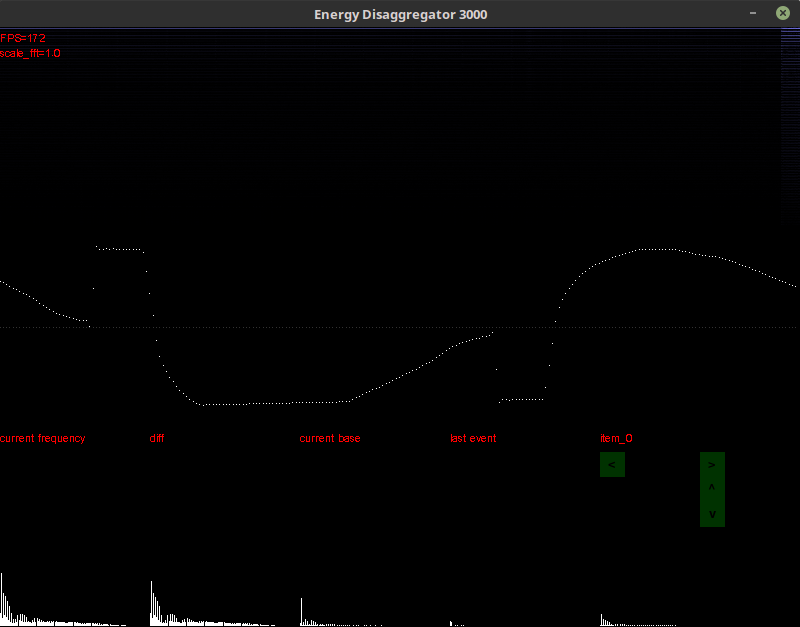
\includegraphics[trim={0 7cm 0 7cm},clip,width=\textwidth,decodearray={1 0 1 0 1 0}]{img/gui-laptop-start.png}
    \caption{Representation of the wave of a laptop charger when just plugged into the laptop and the electrical socket}
    \label{fig:gui-laptop-start}
\end{subfigure}
\begin{subfigure}{\textwidth}
    \centering
    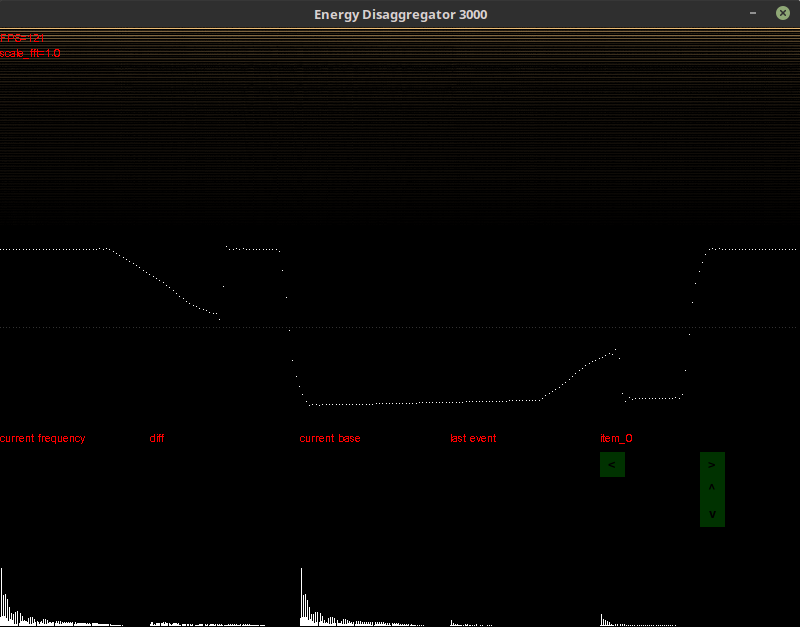
\includegraphics[trim={0 7cm 0 7cm},clip,width=\textwidth,decodearray={1 0 1 0 1 0}]{img/gui-laptop-eco.png}
    \caption{Representation of the wave of a laptop charger after a while when plugged in both laptop and electrical socket}
    \label{fig:gui-laptop-eco}
\end{subfigure}
\begin{subfigure}{\textwidth}
    \centering
    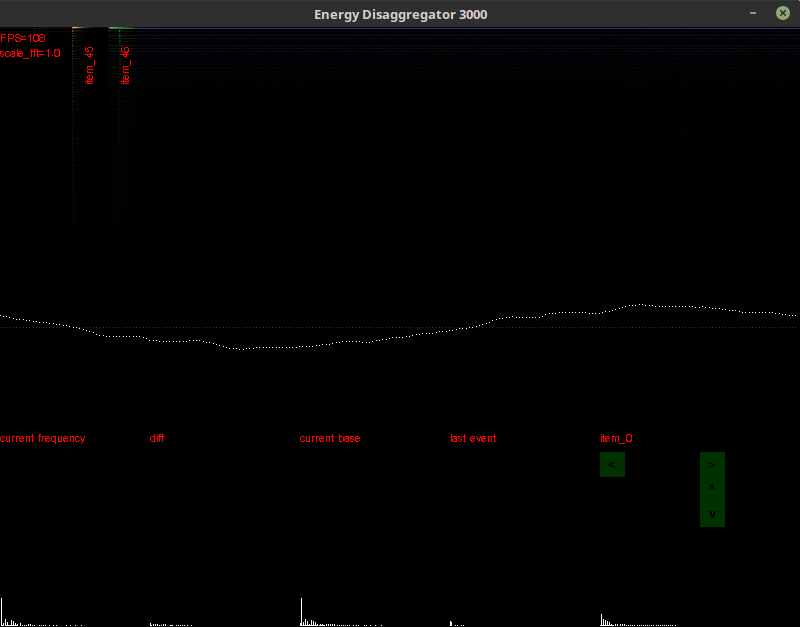
\includegraphics[trim={0 7cm 0 7cm},clip,width=\textwidth,decodearray={1 0 1 0 1 0}]{img/gui-laptop-unplugged.png}
    \caption{Representation of the wave of a laptop charger without plugging it in the laptop}
    \label{fig:gui-laptop-unplugged}
\end{subfigure}
\caption{Representation of the different states of a laptop charger}
\label{fig:gui-laptop}
\end{figure}

\begin{figure}
    \centering
    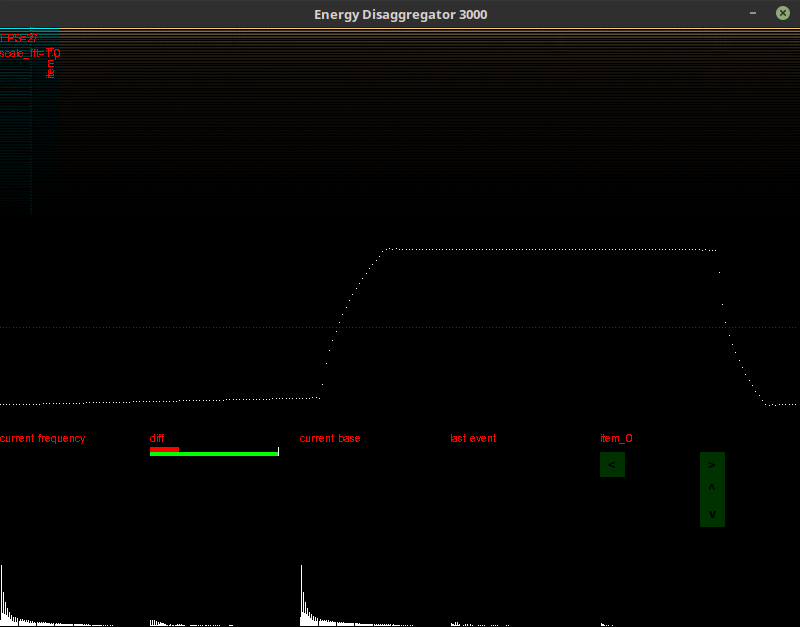
\includegraphics[trim={0 7cm 0 7cm},clip,width=\textwidth,decodearray={1 0 1 0 1 0}]{img/gui-overflow.png}
    \caption{Representation of the wave with a lot of power}
    \label{fig:gui-overflow}
\end{figure}

\subsubsection{Phone Charger}
The phone charger I tested is taking an input of 220V AC with 0.2A, and outputs a 5V DC 1.2A.
I would have expected to see a similar reaction with the phone charger than with the laptop charger but it wasn't exactly the same. Actually there doesn't seem to be a warm-up phase, and when the charger is not connected to the phone, there is almost no current flowing through it and the difference in amplitude is way too small to be detected, this was predictable though since the current flowing in this charger should be 9 times less than for the laptop charger.

\begin{figure}
    \centering
    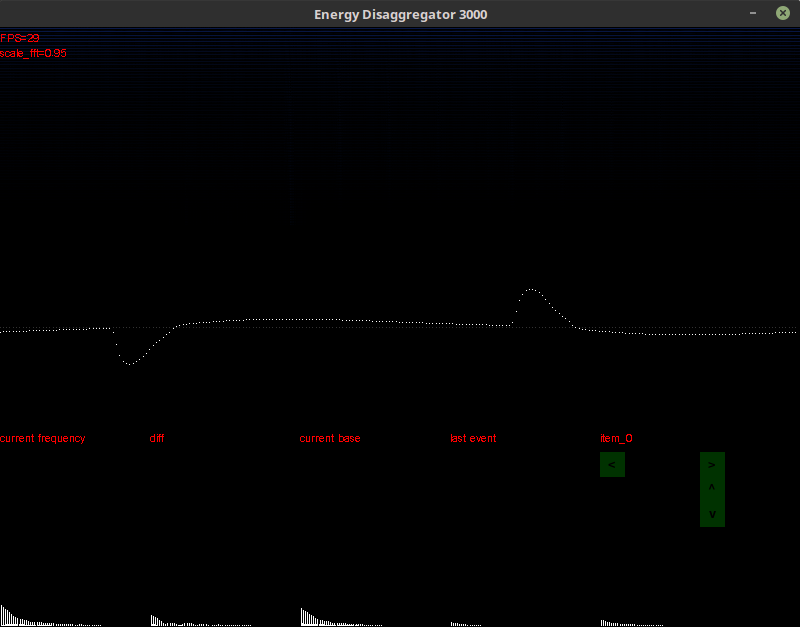
\includegraphics[trim={0 7cm 0 7cm},clip,width=\textwidth,decodearray={1 0 1 0 1 0}]{img/gui-phone.png}
    \caption{Representation of the wave of a phone charger}
    \label{fig:gui-phone}
\end{figure}

